\chapter{Domande per l'Esame}

\qs{}{Come funziona il Transition Based Parser (MALT)?}

\paragraph{Risposta:} si tratta di un tipo di parser che utilizza una grammatica a dipendenze, un algoritmo di ricerca bottom-up e depth-first con oracolo probabilistico.  

\begin{figure}[!h]
    \centering
    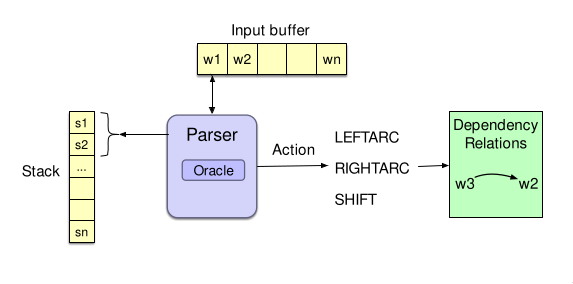
\includegraphics[scale=0.45]{03/parserf.png}
    \caption{Transition-based parsing.}
\end{figure}

\begin{itemize}
  \item \fancyglitter{Stack:} contiene i nodi parzialmente analizzati.
  \item \fancyglitter{Input Buffer:} lista ordinata di parole fornite in input.
  \item \fancyglitter{Dependency Relations:} insieme delle dipendenze analizzate. 
  \item \fancyglitter{Parser:} guarda l'input, guarda sullo stack ed effettua una di tre possibili azioni (operazioni di transizione tra stati):
    \begin{itemize}
      \item LEFTARC: crea un arco a sinistra (tra la parola dell'input e il top dello stack). 
      \item RIGHTARC: crea un arco a destra (tra il top dello stack e la parola dell'input). 
      \item SHIFT: prende la parola in input e la mette nel top dello stack.
    \end{itemize}
\end{itemize}

\cor{Proiettività}{
  IF $i \rightarrow j$ THEN $i \rightarrow * k$ for any $k$ such that $i<k<j$ or $j<k<i$.
}

\nt{In parole povere: se non ci sono incroci.}

\paragraph{Stati:}

\begin{itemize}
  \item \fancyglitter{Stato iniziale:} \{$[$root$]$,$[$sentence$]$, ()\}
  \item \fancyglitter{Stato finale:} \{$[$root$]$,$[$$]$, (R)\} 
    \begin{itemize}
      \item R è l'insieme delle dipendenze costruite. 
      \item  $[]$ è la lista vuota perché tutte le parole sono state analizzate.
    \end{itemize}

\end{itemize}

\paragraph{L'algoritmo:}

\begin{itemize}
  \item Finché lo stato non è finale: 
    \begin{itemize}
      \item Un operatore viene scelto dall'oracolo probabilistico. 
      \item Viene applicato l'operatore effettuando un cambiamento dello stato.
    \end{itemize}
  \item Viene restituito lo stato.
\end{itemize}

\nt{Algoritmo greedy.}

\paragraph{Problemi:}

\begin{itemize}
  \item Tipare le relazioni: aggiungere le relazioni agli operatori, in questo modo si passa da 3 operatori a $2n + 1$ dove $n$ è il numero di relazioni. 
  \item Come capire quale operatore utilizzare: si potrebbe usare un oracolo a regole, ma non è praticabile. Quindi si sceglie si utilizzare un sistema di ML per addestrare un classifier per scegliere l'operatore $\Rightarrow$ si riduce il parsing a un task di classificazione.
\end{itemize}

\qs{}{Cosa è il task della Referring Expression Generation?}

\paragraph{Risposta:} si tratta del task per cui si vuole determinare quali parole usare per esprimere le entità del dominio (nomi propri e pronomi). Spesso si fanno parafrasi per bilanciare fluentezza e ambiguità. 

\qs{}{Spiegare l'uso delle HMM nel PoS Tagging.}

\paragraph{Risposta:} le Hidden Markov Models sono modelli probabilistici utilizzati nel PoS tagging. Sono composte da:

\begin{itemize}
  \item \fancyglitter{Stati nascosti (hidden state):} i tag PoS. 
  \item \fancyglitter{Osservazioni:} le parole nel testo. 
  \item \fancyglitter{Probabilità di transizione:} probabilità che un tag segua un altro. 
  \item \fancyglitter{Probabilità di emissione:} probabilità che una parola appaia dato un tag.
\end{itemize}

\paragraph{Modelling:}

\begin{itemize}
  \item L'obiettivo è trovare la sequenza di tag $\hat{t}_1^n$ che massimizza la probabilità a posteriori:
  \[
  \hat{t}_1^n = \operatorname{argmax}_{t_1^n} P(t_1^n|w_1^n)
  \]
  dove:
  \begin{itemize}
    \item $\hat{t}_1^n$ è la stima della sequenza ottimale di tag
    \item $w_1^n$ rappresenta la sequenza di parole osservate
  \end{itemize}

  \item Applicando il teorema di Bayes e le proprietà delle HMM:
  \[
  P(t_1^n|w_1^n) \propto P(w_1^n|t_1^n) \cdot P(t_1^n) = \prod_{i=1}^n P(w_i|t_i) \cdot P(t_i|t_{i-1})
  \]
  con $t_0 = \text{\texttt{START}}$ (stato iniziale).

  \item Notazioni chiave:
  \begin{itemize}
    \item $\hat{t}$ (hat): stima della migliore sequenza
    \item $\operatorname{argmax}_x f(x)$: valore di $x$ che massimizza $f(x)$
  \end{itemize}

  \item Esempio concreto per una frase di 3 parole:
  \[
  \hat{t}_1^3 = \operatorname{argmax}_{t_1,t_2,t_3} P(t_1)P(t_2|t_1)P(t_3|t_2) \cdot P(w_1|t_1)P(w_2|t_2)P(w_3|t_3)
  \]
\end{itemize}
\paragraph{Learning (Apprendimento dei parametri):}
\begin{itemize}
    \item \fancyglitter{Probabilità di transizione:} 
    $$P(tag_i | tag_{i-1}) = \frac{\text{Conteggio}(tag_{i-1} \rightarrow tag_i)}{\text{Conteggio}(tag_{i-1})}$$
    Esempio: Se \texttt{DET} è seguito da \texttt{NOUN} 70 volte su 100, allora $P(\texttt{NOUN}|\texttt{DET}) = 0.7$.

    \item \fancyglitter{Probabilità di emissione:} 
    $$P(parola | tag) = \frac{\text{Conteggio}(parola \text{ con } tag)}{\text{Conteggio}(tag)}$$
    Esempio: Se la parola "cane" appare 90 volte come \texttt{NOUN}, $P(\texttt{"cane"}|\texttt{NOUN}) = 0.9$.

    \item \fancyglitter{Probabilità iniziali:} 
    $$P(tag_1) = \frac{\text{Conteggio}(tag_1 \text{ come primo tag})}{\text{Totale frasi}}.$$
\end{itemize}

\paragraph{Decoding (Assegnazione dei tag):}
L'algoritmo di Viterbi seleziona la sequenza di tag $\hat{t}_1^n$ che massimizza:
$$\argmax_{t_1^n} P(t_1^n | w_1^n) \propto \prod_{i=1}^n P(t_i | t_{i-1}) \cdot P(w_i | t_i),$$
dove:
\begin{itemize}
    \item $t_i$ è il tag alla posizione $i$,
    \item $w_i$ è la parola alla posizione $i$.
\end{itemize}

\qs{}{Che differenza c'è tra MEMM e HMM?}

\paragraph{Risposta:} I modelli MEMM (Maximum Entropy Markov Models) e HMM (Hidden Markov Models) sono approcci probabilistici diversi per il tagging sequenziale. Le differenze principali sono:

\begin{center}
\begin{tabular}{|l|l|l|}
\hline
\textbf{Aspetto} & \textbf{HMM} & \textbf{MEMM} \\
\hline
\fancyglitter{Modello probabilistico} & Generativo & Discriminativo \\
\hline
\fancyglitter{Probabilità modellate} & $P(W,T) = \prod P(w_i|t_i)P(t_i|t_{i-1})$ & $P(T|W) = \prod P(t_i|t_{i-1},w_i)$ \\
\hline
\fancyglitter{Feature} & Solo parole e tag & Feature arbitrarie (es: prefissi, suffissi) \\
\hline
\fancyglitter{Problema noto} & Independence assumptions & Label bias problem \\
\hline
\fancyglitter{Efficienza} & $O(nT^2)$ (Viterbi) & $O(nT^2)$ (Viterbi modificato) \\
\hline
\end{tabular}
\end{center}

\paragraph{Dettagli chiave:}

\begin{itemize}
\item \fancyglitter{Natura dei modelli:}
\begin{itemize}
\item Gli HMM sono \textit{generativi}: modellano la probabilità congiunta $P(W,T)$
\item I MEMM sono \textit{discriminativi}: modellano direttamente $P(T|W)$
\end{itemize}

\item \fancyglitter{Flessibilità:}
\begin{itemize}
\item Gli HMM usano solo emissioni $P(w|t)$ e transizioni $P(t_i|t_{i-1})$
\item I MEMM possono incorporare feature complesse (es: "La parola finisce con '-mente'")
\end{itemize}

\item \fancyglitter{Problemi intrinseci:}
\begin{itemize}
\item HMM soffre di \textit{independence assumptions} (emissioni indipendenti dal contesto)
\item MEMM soffre di \textit{label bias} (tendenza a preferire stati con meno transizioni)
\end{itemize}

\item \fancyglitter{Esempio di feature in MEMM:}
\[
P(t_i|t_{i-1},w_i) = \frac{1}{Z}\exp\left(\sum_j \lambda_j f_j(t_i,t_{i-1},w_i)\right)
\]
dove $f_j$ sono feature (es: "la parola è maiuscola?") e $\lambda_j$ pesi appresi.
\end{itemize}
\qs{}{Dove si trovano le lingue naturali nella gerarchia di Chomsky?}

\paragraph{Risposta:} sono \fancyglitter{Mildly Context-Sensitive} ($a^n b^n c^n$) e si collocano tra le Context-Sensitive ($a^{2^n}$) e le Context-free ($a^n b^n$).

\qs{}{Cosa è una probabilistic CFG?}

\paragraph{Risposta:} una probabilistic CFG è una distribuzione di probabilità sulle regole di una grammatica. La somma dei valori dei lati destri di una regola (dato il suo lato sinistro) deve fare 1. 

\qs{}{Che cosa è il realizer nella NLG?}

\paragraph{Risposta:} Il \fancyglitter{realizer} (o \textit{surface realizer}) è il componente fondamentale di un sistema di Natural Language Generation (NLG) che trasforma una rappresentazione astratta del contenuto (tipicamente strutture sintattiche o semantiche) in testo linguisticamente corretto e fluente. 

\paragraph{Funzionamento del realizer:}
\begin{itemize}
  \item \fancyglitter{Input:} Riceve una rappresentazione intermedia (es: \textit{deep syntax} o \textit{semantic graphs})
  \item \fancyglitter{Output:} Genera frasi grammaticalmente corrette nella lingua target
  \item \fancyglitter{Processi chiave:}
  \begin{itemize}
    \item \textbf{Linearizzazione}: Disposizione ordinata delle parole
    \item \textbf{Morfologia}: Flessione di genere, numero, tempo verbale
    \item \textbf{Surface realization}: Scelta di articoli/preposizioni (es: "al" vs "allo")
    \item \textbf{Orthographic realization}: Capitalizzazione, punteggiatura
  \end{itemize}
\end{itemize}

\paragraph{Esempio concreto:}
\begin{itemize}
  \item \textbf{Input}: 
  \begin{verbatim}
    (AGGIUNGI (OGGETTO "libro") 
    (ATTRIBUTI (COLORE "rosso") (POSIZIONE "scrivania"))
  \end{verbatim}
  \item \textbf{Output}: \textit{"Aggiungi il libro rosso sulla scrivania"}
\end{itemize}

\paragraph{Tecnologie utilizzate:}
\begin{itemize}
  \item \fancyglitter{Grammar-based}: Realizer con grammatiche hand-crafted (es: FUF/SURGE)
  \item \fancyglitter{Statistical}: Modelli neurali (LSTM/Transformer) addestrati su corpora
  \item \fancyglitter{Hybrid}: Combinazione di regole e modelli statistici
\end{itemize}

\paragraph{Strumenti noti:}
\begin{itemize}
  \item \textbf{SimpleNLG}: Libreria Java per realizzazione in inglese/francese
  \item \textbf{GRAMLEX}: Sistema per flessione morfologica italiana
  \item \textbf{OpenCCG}: Realizer basato su grammatiche categoriali
\end{itemize}

\qs{}{Cosa è il task dell'Aggregation?}

\paragraph{Risposta:} L'\fancyglitter{Aggregation} è un task fondamentale nella Natural Language Generation (NLG) che combina multiple unità d'informazione in strutture linguistiche più complesse e naturali, riducendo la ridondanza e migliorando la fluidità del testo generato.

\qs{}{Elencare i 5 algoritmi per il parsing delle dipendenze sintattiche.}

\paragraph{Risposta:}

\begin{itemize}
  \item Dynamic Programming (simile a CKY): Ha complessità $O(n^5)$, ma Eisner ne ha scoperto uno con complessità $O(n^3)$. 
  \item Graph Algorithm: si crea un minimum spanning tree e vengono valutate le dipendenze in modo indipendente utilizzando un ML classifier. 
  \item Constituency Parsing: si fa il parsing con una grammatica a costituenti e si converte in una grammatica a dipendenze attraverso una \fancyglitter{tabella di percolazioni}.
  \item Transition-based parsing (MALT): anche detto deterministico. Si fanno scelte greedy per la creazione di dipendenze tra parole, guidate da ML classifier.
  \item Constraint Satisfaction: vengono eliminate tutte le possibili dipendenze che non soddisfano certi vincoli (un esempio è TUP).
\end{itemize}

\qs{}{Quali sono i task della NLG?}

\paragraph{Risposta:}

\begin{enumerate}
  \item \fancyglitter{Content determination:} 
    \begin{itemize}
      \item Messaggi provenienti da una struttura dati. 
      \item I messaggi sono aggregazioni di dati che possono essere espressi linguisticamente, con una parola o un sintagma. 
      \item I messaggi sono basati su entità, concetti e relazioni sul dominio. Non c'è nulla di linguistico.  
      \item \evidence{Esempio:} IDENTITY(NEXTTRAIN, CALEDONIANEXPRESS); The next train is the Caledonian Express.
      \item \evidence{Esempio:} DEPARTURETIME(CALEDONIANEXPRESS, 1000); The Caledonian Express leaves at 10am. 
      \item \evidence{Esempio:} COUNT((TRAIN, SOURCE(ABERDEEN),DESTINATION(GLASGOW)), 20, PERDAY); There are 20 trains daily from Aberdeen to Glasgow.
    \end{itemize}
  \item \fancyglitter{Discourse planning:}
    \begin{itemize}
      \item Un testo non è solo un collezione casuale di frasi. 
      \item C'è una struttura che relaziona le frasi. 
      \item Due tipi di relazione:
        \begin{itemize}
          \item Raggrupamento concettuale. 
          \item Relazioni retoriche.
        \end{itemize}
      \item \evidence{Esempio:}
\begin{figure}[h]
    \centering
    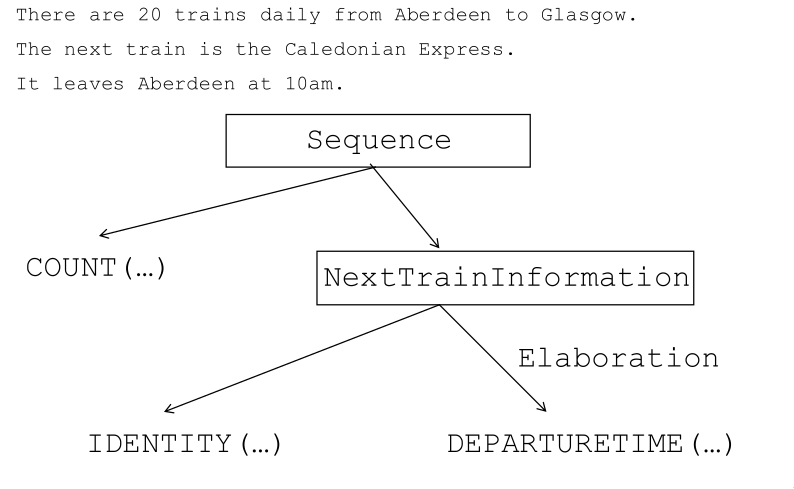
\includegraphics[scale=0.4]{06/dp.png}
\end{figure}

    \end{itemize}
  \item \fancyglitter{Sentence Aggregation:}
    \begin{itemize}
      \item Se si dicessero tutte le frasi 1-a-1 si avrebbe un discorso poco naturale e non fluente. 
      \item Per questo motivo i messaggi vengono combinati per formare frasi più complesse. 
      \item Può causare ambiguità, ma ci si aspetta che l'altro sappia disambiguare.
      \item È il primo task che dipende dalla lingua.
      \item \evidence{Esempio:} The next train, which leaves at 10 am, is the Caledonian Express.
    \end{itemize}
  \item \fancyglitter{Lexicalization:} 
    \begin{itemize}
      \item Determina: 
        \begin{itemize}
          \item Quali parole usare per esprimere i concetti e le relazioni del dominio. 
          \item Quali relazioni sintattiche tra le parole.
        \end{itemize}
      \item \evidence{Esempio:} si deve usare partire o decollare?
    \end{itemize}
  \item \fancyglitter{Referring Expression Generator:}
    \begin{itemize}
      \item Generare le “referrinhg expressions” determina quali parole usare per esprimere le entità del dominio in una maniera comprensibile all'utente. 
      \item Si bilancia fluentazza e ambiguità (a volte con parafrasi).
      \item \evidence{Esempio:} 
        \begin{itemize}
          \item Aberdeen, Scotland. 
          \item Aberdeen.
        \end{itemize}
      \item \evidence{Esempio:}
        \begin{itemize}
          \item The train that leaves at 10am. 
          \item The next train.
        \end{itemize}
    \end{itemize}
  \item \fancyglitter{Syntactic and morphological realization:}
    \begin{itemize}
      \item Ogni lingua ha: 
        \begin{itemize}
          \item Morfologia: come si formano le parole. 
          \item Sintassi: come si formano le frasi.
        \end{itemize}
      \item Arrivati a questo livello il dominio non ha più alcuna importanza, è tutta linguistica.
    \end{itemize}
  \item \fancyglitter{Orthographic realization:} 
    \begin{itemize}
      \item Lettere grandi. 
      \item Punteggiatura. 
      \item Font. 
      \item Impaginazione.
    \end{itemize}
\end{enumerate}


\qs{}{Spiegare l'uso del formalismo lambda-FoL per la semantica computazionale.}

\paragraph{Risposta:} si usa la logica del prim'ordine (FoL) per poter ragionare sul linguaggio in maniera automatica. Tuttavia la FoL non permette di rappresentare alcune cose (predicati universali), per cui si introduce la lambda astrazione. Il motivo è che serve poter avere delle funzioni.

\nt{Maggiori informazioni nell'apposita sezione.}

\qs{}{Cosa è la rappresentazione Neo-Davidsoniana?}

\paragraph{Risposta:} una rappresentazione che usa FoL in cui si reificano gli eventi, ossia si definisce una variabile per identificare l'evento.

\qs{}{Quali sono le due ipotesi fondamentali della linguistica computazionale?}

\paragraph{Risposta:} La linguistica computazionale poggia su due ipotesi fondamentali che ne guidano l'approccio teorico e metodologico:

\paragraph{1. \fancyglitter{Ipotesi discreta del linguaggio}}
\begin{itemize}
  \item Postula che il linguaggio sia costituito da \textbf{unità discrete} (fonemi, morfemi, parole) combinabili secondo regole
  \item Implicazioni computazionali:
  \begin{itemize}
    \item Rappresentabilità mediante strutture formali (grammatiche, automi)
    \item Segmentazione precisa di testi/token (es: word boundary detection)
    \item Modellazione come processi Markoviani (catene di stati discreti)
  \end{itemize}
  \item Contro-esempi da gestire:
  \begin{itemize}
    \item Fenomeni continui (es: intonazione, gradazioni semantiche)
    \item Casi di ambiguità segmentativa (es: "l'ago" vs "la go")
  \end{itemize}
\end{itemize}

\paragraph{2. \fancyglitter{Ipotesi della computabilità linguistica}}
\begin{itemize}
  \item Assume che i processi linguistici siano \textbf{algoritmicamente modellabili}
  \item Conseguenze operative:
  \begin{itemize}
    \item Sviluppo di parser per grammatiche formali (es: CFG, TAG)
    \item Apprendimento automatico di pattern linguistici
    \item Decidibilità dei problemi linguistici (es: membership problem)
  \end{itemize}
  \item Limiti teorici:
  \begin{itemize}
    \item Problemi NP-completi per grammatiche espressive
    \item Trade-off tra copertura linguistica e complessità computazionale
  \end{itemize}
\end{itemize}

\paragraph{Interazione tra le ipotesi:}
\[
\text{Discretezza} \Rightarrow \text{Rappresentabilità formale} \Rightarrow \text{Computabilità}
\]

\qs{}{Cosa è la frame-based semantic nei DS?}

\paragraph{Risposta:} in un dialogue system si hanno dei frames che vanno riempiti con informazioni che vanno ricavate dal dialogo con l'utente. 

\nt{Vedere apposita sezione per più dettagli.}

\qs{}{Fare un esempio di ambiguità puramente semantica.}

\paragraph{Risposta:} ho visto l'uomo sul monte con il telescopio.

\qs{}{Ambiguità sintattica: spiegare i fenomeni del PP attachment e dell'ambiguità sintattica.}

\paragraph{Risposta:} L'\fancyglitter{ambiguità sintattica} si verifica quando una frase ammette molteplici analisi strutturali, con significati potenzialmente diversi. Una PP può modificare diversi costituenti.

\paragraph{Esempio canonico:}
\textit{"Ho visto l'uomo con il telescopio"}

\begin{itemize}
  \item \fancyglitter{Interpretazione 1} (attacco al VP):
  \begin{itemize}
    \item Struttura: [VP [V visto] [NP l'uomo] [PP con il telescopio]]
    \item Significato: L'osservatore usa il telescopio
    \item Rappresentazione: $\lambda e.\,\text{vedere}(e) \land \text{Agente}(e,\text{io}) \land \text{Strumento}(e,\text{telescopio})$
  \end{itemize}

  \item \fancyglitter{Interpretazione 2} (attacco all'NP):
  \begin{itemize}
    \item Struttura: [VP [V visto] [NP l'uomo [PP con il telescopio]]]
    \item Significato: L'uomo possiede il telescopio
    \item Rappresentazione: $\lambda e.\,\text{vedere}(e) \land \text{Agente}(e,\text{io}) \land \text{Possessore}(\text{uomo},\text{telescopio})$
  \end{itemize}
\end{itemize}
\qs{}{Come funziona l'algoritmo CKY?}

\nt{Vedere l'apposità sezione.}

\qs{}{Qual è la complessità dell'algoritmo CKY rispetto alla lunghezza N dell'input?}

\paragraph{Risposta:} $O(n^3)$ per la versione non probabilistica, $O(n^5)$ per la versione probabilistica. 

\qs{}{Che differenza c'è tra la sintassi formalizzata come dipendenze e quella come costituenti?}

\paragraph{Risposta:} differiscono per la struttura, quella a costituenti forma degli alberi, quella a dipendenze crea collegamenti tra varie parole.

\qs{}{Che cos'è la misura PARSEVAL?}

\paragraph{Risposta:} si tratta di uno standard di valutazione per parser sintattici per confrontare alberi di costituenza generati automaticamente con alberi di riferimento (gold).

\qs{}{Che cos'è un treebank?}

\paragraph{Risposta:} un treebank è un corpus che annota la struttura sintattica o semantica di molte frasi.

\qs{}{Quali sono le fasi della NLG simbolica?}

\paragraph{Risposta:} La NLG simbolica tradizionale segue una pipeline modulare composta da sei fasi fondamentali, secondo il modello \fancyglitter{Reiter \& Dale} (2000):

\begin{enumerate}
\item \fancyglitter{Content Determination}
\begin{itemize}
    \item \textbf{Scopo}: Selezionare le informazioni da verbalizzare
    \item \textbf{Input}: Knowledge base o dati strutturati
    \item \textbf{Output}: Insieme di proposizioni logiche
    \item \textbf{Esempio}: Da DB meteo a $\{\text{temp}(oggi, 22°C), \text{pioggia}(domani, 80\%)\}$
\end{itemize}

\item \fancyglitter{Document Planning}
\begin{itemize}
    \item \textbf{Scopo}: Organizzare la struttura del discorso
    \item \textbf{Sottofasi}:
    \begin{itemize}
        \item \textit{Macroplanning}: Ordinamento delle informazioni
        \item \textit{Microplanning}: Raggruppamento concettuale
    \end{itemize}
    \item \textbf{Tecniche}: Rhetorical Structure Theory (RST)
\end{itemize}

\item \fancyglitter{Lexicalization}
\begin{itemize}
    \item \textbf{Scopo}: Mappare concetti a parole
    \item \textbf{Decisioni}:
    \begin{itemize}
        \item Scelta lessicale (\textit{"acquistare"} vs \textit{"comprare"})
        \item Classi di parole (verbo vs nominalizzazione)
    \end{itemize}
    \item \textbf{Risorse}: Ontologie lessicali (WordNet)
\end{itemize}

\item \fancyglitter{Referring Expression Generation}
\begin{itemize}
    \item \textbf{Scopo}: Introdurre entità nel discorso
    \item \textbf{Strategie}:
    \begin{itemize}
        \item Forme definite (\textit{"il libro"})
        \item Descrizioni (\textit{"il romanzo pubblicato nel 2020"})
        \item Pronominalizzazione
    \end{itemize}
    \item \textbf{Algoritmi}: Full Brevity, Incremental
\end{itemize}

\item \fancyglitter{Aggregation}
\begin{itemize}
    \item \textbf{Scopo}: Combinare proposizioni
    \item \textbf{Operazioni}:
    \begin{itemize}
        \item Coordinazione (\textit{"e"})
        \item Subordinazione (\textit{"perché"})
        \item Ellissi
    \end{itemize}
    \item \textbf{Esempio}: \textit{"La temperatura è 22°C"} + \textit{"Il cielo è sereno"} → \textit{"La temperatura è 22°C con cielo sereno"}
\end{itemize}

\item \fancyglitter{Linguistic Realization}
\begin{itemize}
    \item \textbf{Scopo}: Generare la superficie linguistica
    \item \textbf{Compiti}:
    \begin{itemize}
        \item Flessione morfologica
        \item Ordinamento parole
        \item Inserimento articoli/preposizioni
    \end{itemize}
    \item \textbf{Strumenti}: Realizer come SimpleNLG
\end{itemize}
\end{enumerate}
\qs{}{HMM è un modello generativo o discriminativo?}

\paragraph{Risposta:} HMM è un modello generativo: per capire se in una foto c'è un cane si guardano le caratteristiche che lo rendono un cane (e.g. la code, etc.). MEMM invece è discriminativo: se si vede un guinzaglio non è un cane. 

\qs{}{Spiegare cosa si intende per anatomia di un parser.}

\paragraph{Risposta:}

\begin{itemize}
  \item Grammatica o modello di automa. 
  \item Algoritmo:
    \begin{itemize}
      \item Strategia di ricerca. 
      \item Organizzazione della memoria.
    \end{itemize}
  \item Oracolo.
\end{itemize}

\qs{}{Quali sono i 6 fenomeni del dialogo tra umani?}

\paragraph{Risposta:}

\begin{itemize}
  \item \fancyglitter{Turni:} 
    \begin{itemize}
      \item Ogni contributo alla conversazione. 
      \item È come se la comunicazione venisse vista come un gioco.  
      \item Il problema del turno: Come si capisce quando prendere il turno? Si può concedere all'utente di interrompere il sistema. La difficoltà sta nella comprensione del sistema, poiché può capitare che le persone smettano di parlare temporanemente nel proprio turno.
    \end{itemize}
    \fancyglitter{Speech Acts:}
    \begin{itemize}
      \item Constativi: affermare qualcosa.
      \item Direttivi: tentativo del parlante di far fare qualcosa all'altra persona.
      \item Committivi: riguardanti azioni future del parlante.
      \item Riconoscitivi: esprire un'attitudine riguardo la persona che sta ascoltando.
    \end{itemize}
    \fancyglitter{Grounding:}
    \begin{itemize}
      \item I partecipanti alla conversazione hanno bisogno di un "terreno comune". 
      \item Consiste nel confermare che l'ascoltatore abbia capito. 
      \item Esempio: il bottone di un ascensore che si illumina\footnote{Tranne in dipartimento I guess.}.
    \end{itemize}
    \fancyglitter{Struttura del Dialogo:}
    \begin{itemize}
      \item \evidence{Punti di Adiacenza:} si ha una struttura sensata. 
      \item Domanda e Risposta. 
      \item Proposta e Accettazione/Rifiuto.
    \item \evidence{Sottodialoghi:} il dialogo può specializzarsi in un sottodialogo collegato e poi ritonare al punto da cui si è partiti (struttura ricorsiva). 
    \item \evidence{Presequenza:} chiedere un qualcosa e successivamente confermarlo.
    \end{itemize}
  \item \fancyglitter{Iniziativa:}
    \begin{itemize}
      \item Alcune conversazioni sono controllate da una sola persona. 
      \item Ma diverse conversazioni umane hanno un'iniziativa mista. 
      \item Tuttavia questo è difficile da replicare per cui solitamente si ricorre o all'iniziativa dell'utente (da cui derivano i vari ChatBOTs) o all'iniziativa del sistema (il sistema guida la conversazione su binari prestabiliti). 
    \end{itemize}
  \item \fancyglitter{Inferenza:}
    \begin{itemize}
      \item Da ciò che viene detto si deve ricavare il significato. 
      \item I principi di inferenza sulle conversazioni di Grice (principio di massima rilevanza, etc.).
    \end{itemize}
\end{itemize}


\qs{}{Cos'è il PoS Tagging?}

\paragraph{Risposta:} il Part of Speech tagging è il task in cui si fornisce in input una frase e viene restituita in output una frase taggata con le varie parti della frase (NOUN, VERB, ADJ, etc.). Molte parole sono ambigue (hanno più PoS associati), quindi è necessario disambiguare con un algoritmo. Il 60\% dei token sono ambigui. 

\paragraph{È importante perché:}

\begin{itemize}
  \item La pronuncia di parole dipende dal PoS. 
  \item Serve per analisi di Noun Phrases (shallow parsing). 
  \item Serve per l'analisi sintattica. 
  \item Per Machine Translation (con lingue simili). 
  \item Per sentiment analysis. 
  \item Da un punto di vista linguistico: capire le parti più utilizzate e quando.
\end{itemize}

\qs{}{Cos'è il NER Tagging?}

\paragraph{Risposta:} il Named Entities recognition è un task di tagging che si applica unicamente ai nomi propri. Per distinguere se indicano persone, organizzazioni, luoghi, etc. A differenza del PoS tagging è un multi word: New York City, Marie Curie, etc. 

\paragraph{2 Sottotask:}

\begin{itemize}
  \item Trovare lo span di testo che costituisce i nomi propri. 
  \item Taggare il tipo di entità.
\end{itemize}

\paragraph{Perché si vuole fare NER?}

\begin{itemize}
  \item Sentiment analysis: i sentimenti di un consumatore verso un prodotto. 
  \item Q\&A: rispondere a domande su entità. 
  \item Information extraction: estrarre fatti su entità da un testo.
\end{itemize}

\paragraph{Come si fa?}

\begin{itemize}
  \item BIO Tagging: Begin Inside Outside.
  \item L'idea è che ci si segna l'inizio (begin), quando si è dentro (inside) e quando si esce (outside).
  \item I tag necessari sono $2n + 1$ dove $n$ è il numero di diverse NE possibili.
\end{itemize}

